\chapter{Amplifier Circuits}
It was researched some types of amplifiers circuits, it was selected the circuits
with single supply, because the project was designed to be the maximum embedded
on the guitar, without the needing of other supplies except the guitar battery
or the USB connection of the microprocessor.
After some researches it was decided try two circuit types, with two different
operational amplifiers. The first circuit uses the Texas Instruments INA 326
Instrumental Amplifier and the second uses the Texa Instruments TLV 4316 Operational Amplifier.

\section{INA 326}
The project using the INA 326 IC, started with a research at the datasheet of
this compnent and it was verified one circuit which provides the desired Gain to
the electric signal from the pickup respecting the project's initial requests.
The circuit is shown on figure 3.

\begin{figure}[!htpb]
\centering
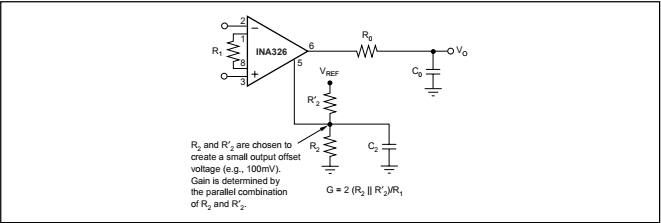
\includegraphics[scale=0.8]{images/Texas}
\caption{Amplifier assembly}
\end{figure}

This circuit amplifies the signal and the gain is obtained by the following equation:

$$G=2*\frac{(R_2||R_2 ')}{R_1}$$

On the project the Resistor $R_0$ and the Capacitor $C_0$ was excluded because
it was not relevant on the output to this project. After the research it was
developed a schematic model to perform some simulation tests to verify and prove
the functionalism of the circuit for the desired application. The schematic circuit
it was developed using the software CadSoft Eagle Professional 7.6.0 until the version
showed at figure 4.

\begin{figure}[!htpb]
\centering
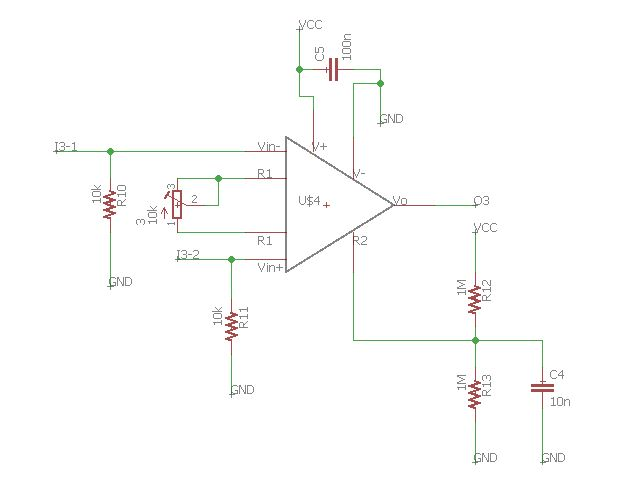
\includegraphics[scale=0.7]{images/INA}
\caption{Schematic for each channel}
\end{figure}

This circuit as showed on the image provides a Gain of:

$$G=2*\frac{(1M\Omega||1M\Omega)}{10k\Omega}$$
$$G=2*\frac{500k\Omega}{10k\Omega}$$
$$G=2*50$$
$$G=100$$

The amplifier circuit was projected to each channel. So the circuit needed 6 IC
INA 326 to be complete. The complete schematic is showed on annex 1. After project
the schematic circuit to each channel it was developed the PCB project, using the
same software described on the schematic modelling. The PCI project is showed on figure 5.\\

This PCB project was projected on a dual layer board scheme, using 15 mils of
minimum width for the conductive tracks. It was assembled on FR4 dual layer copper
board, combining the through-hole and surface-mount technologies. This choice was
made due the facility of the assembly of the through-hole components. It was sent
the files to one person who works with printing PCB boards. After the processes
the PCB was like figure 6.\\

\begin{figure}[!htpb]
\centering
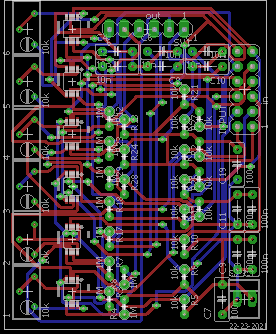
\includegraphics[scale=1.5]{images/TCC_INA}
\caption{PCB Project}
\end{figure}

\begin{figure}[!htpb]
\centering
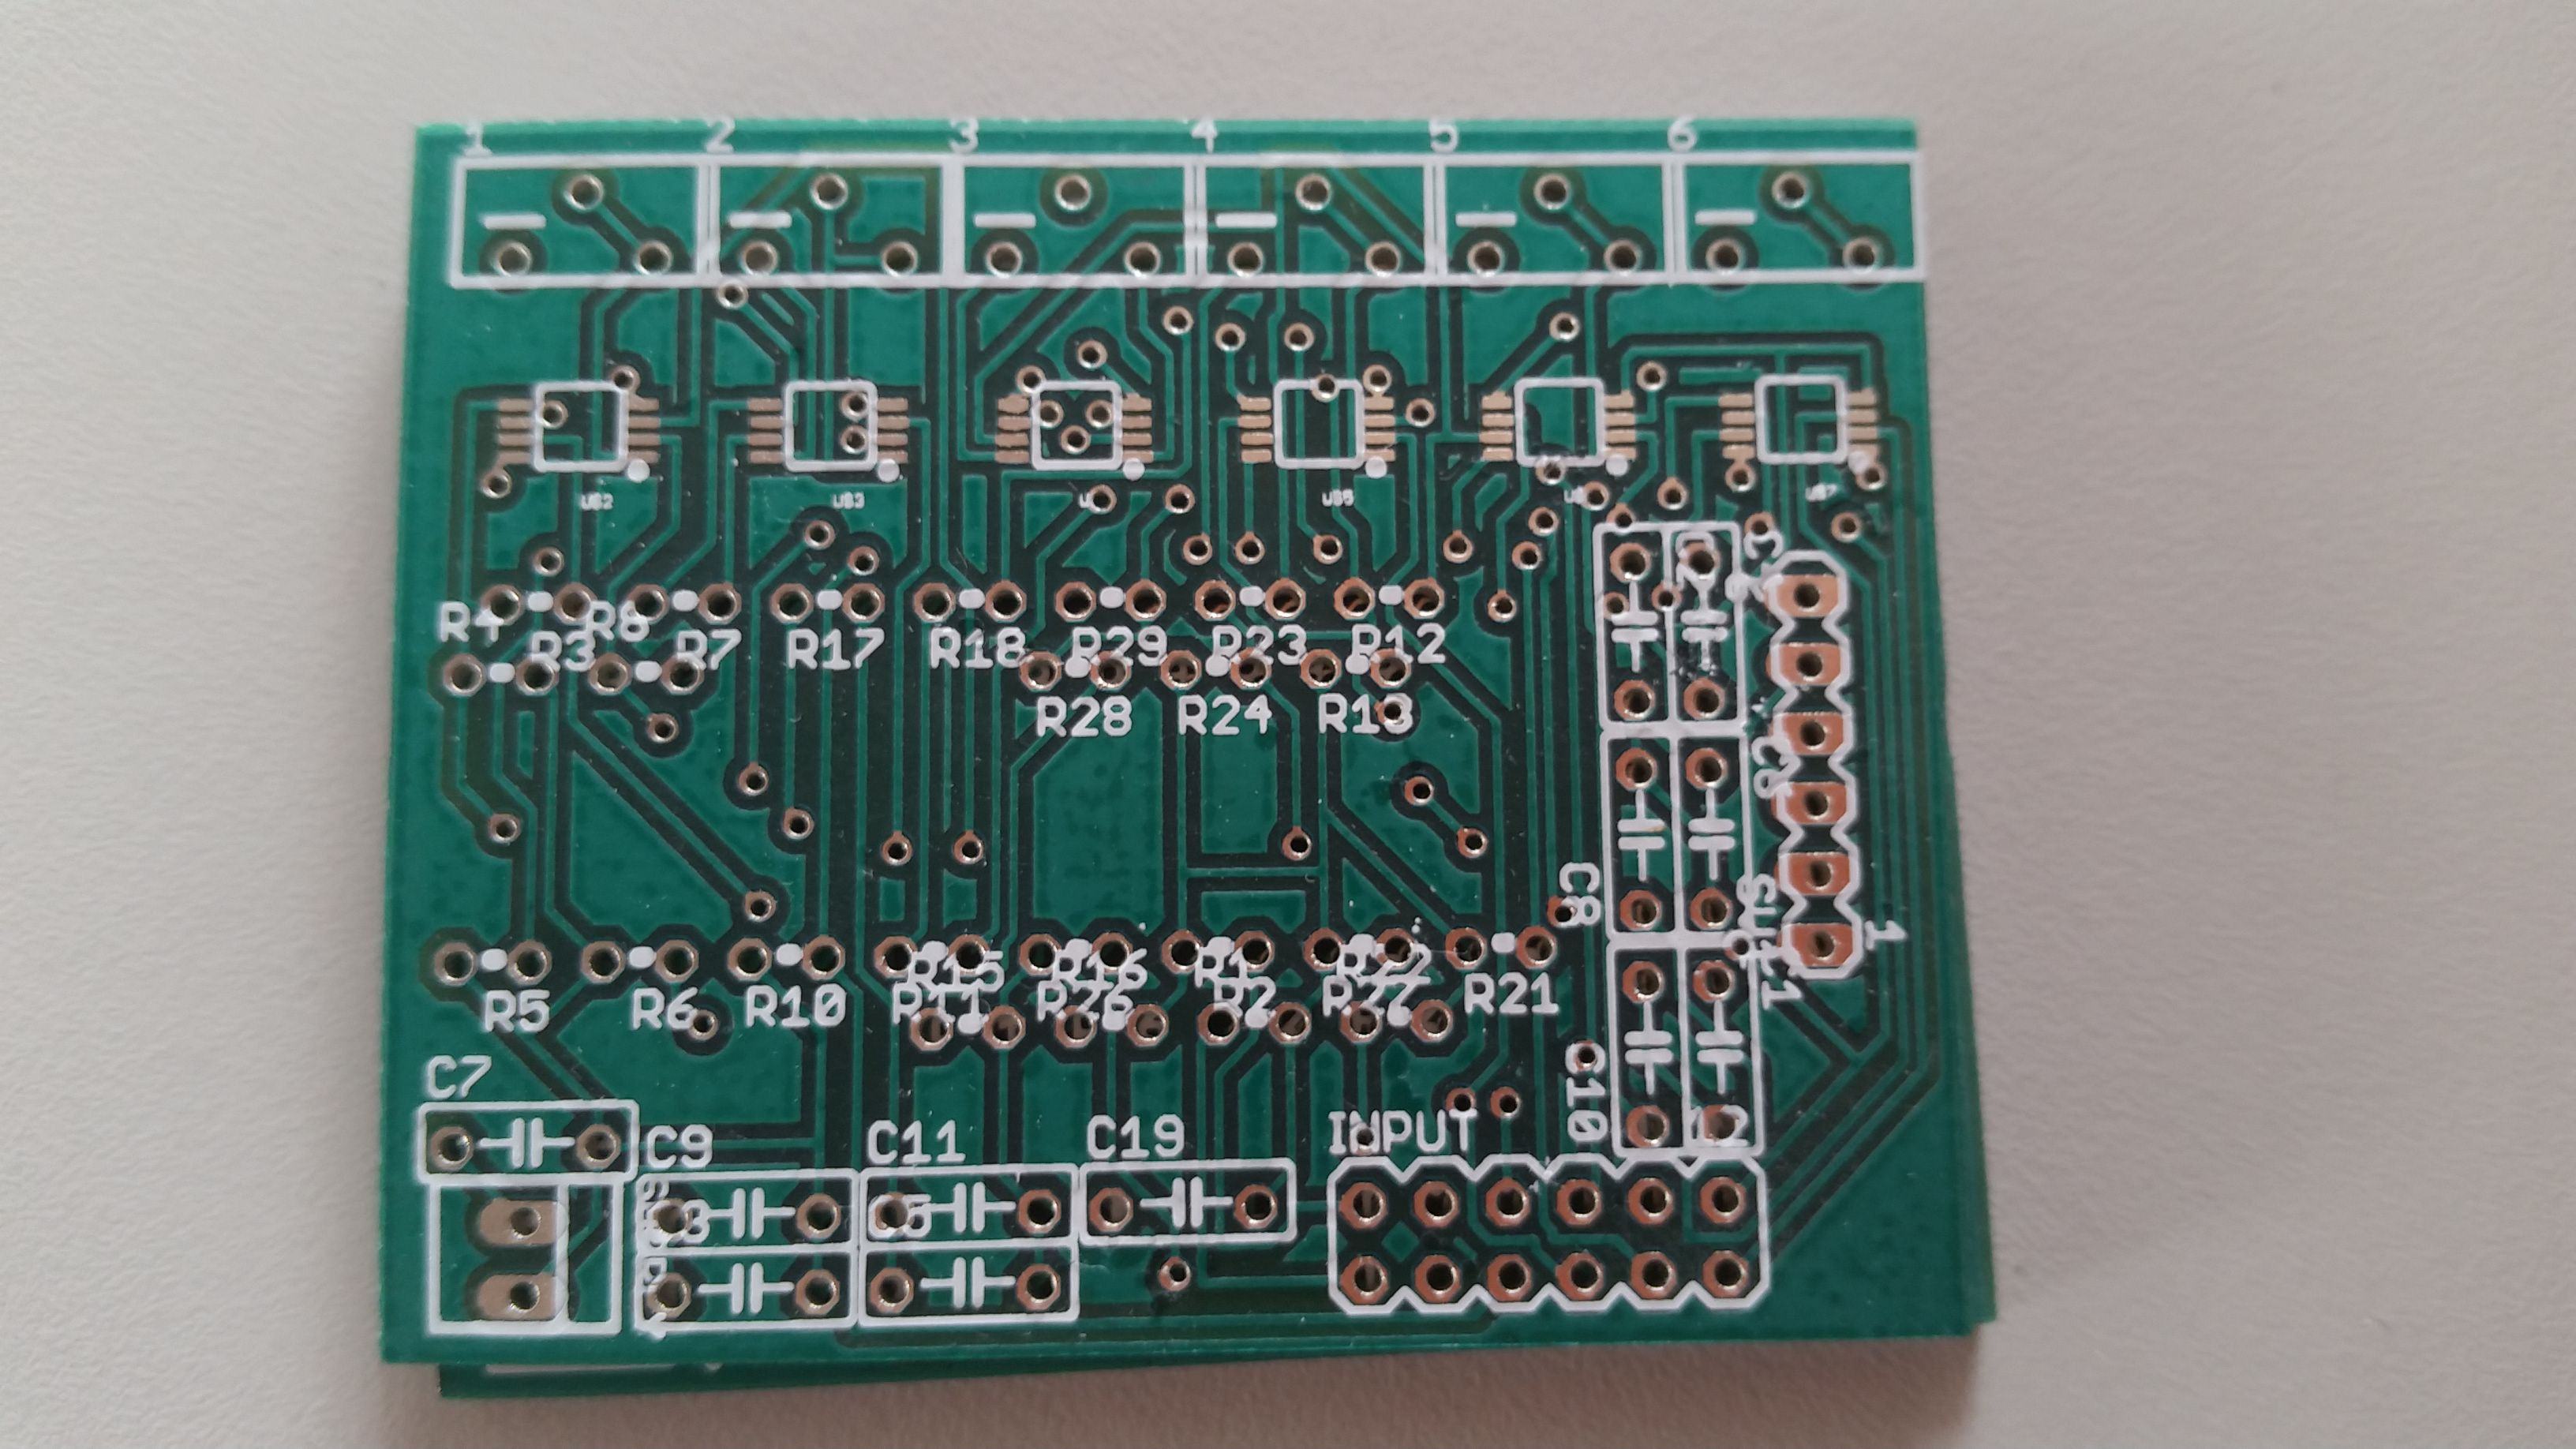
\includegraphics[scale=0.08]{images/INA_board}
\caption{PCB Project}
\end{figure}

On this project it was used:

\begin{itemize}
\item 6 Instrumental Amplifiers INA 326;
\item 6 10k$\Omega$ Trimmer Potentiometer;
\item 6 10nF Ceramic Capacitor;
\item 6 100nF x 50V Electrolitic Capacitor;
\item 12 10k$\Omega$ 5 Percent Tolerance Resistor;
\item 12 1M$\Omega$ 5 Percent Tolerance Resistor;
\item 1 6 positions Pin bar;
\item 1 12 positions dual track Pin bar;
\item 1 2 positions Pin bar;
\end{itemize}

After soldering all the components it was performed some bench tests to
verify the functionality of the amplifier circuit. The result showed us that the
circuit attends the required function, amplifying the signal from a pick of 10mV
to a pick of 1V, proving that the circuit is working perfectly and attending the
demand of the project. After the bench test the system was connected to the pickup
to verify if the guitar signal would be amplified as needed to the conversion process.
The result was satisfactory and attended well the purpose to the project, as showed on image 6.

\begin{figure}[!htpb]
\centering
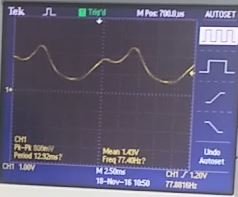
\includegraphics[scale=1]{images/INA_result}
\caption{INA Project Result}
\end{figure}

\section{TLV 4316}
The project of TLV 4316 started on the same way of the INA 326 project.
It started verifying the datasheet
